%% ============================================================
%%  IEEE Transactions — artículo en español
%%  Compilador: pdfLaTeX  (Overleaf: default)
%% ============================================================
\documentclass[journal,12pt,onecolumn]{IEEEtran}

% ── Paquetes ──────────────────────────────────────────────────
\usepackage[T1]{fontenc}
\usepackage[utf8]{inputenc}
\usepackage[spanish,es-nodecimaldot]{babel}
\usepackage{amsmath,amssymb,bm}
\usepackage{graphicx}
\usepackage{booktabs}
\usepackage{array}
\usepackage{url}
\usepackage{hyperref}
% siunitx/algorithm/cite/balance reemplazados con macros mínimas
\newcommand{\SI}[2]{\ensuremath{#1\,\mathrm{#2}}}
\newcommand{\si}[1]{\ensuremath{\mathrm{#1}}}

% ── Rutas de figuras ──────────────────────────────────────────
\graphicspath{{../results/figures/}{../assets/}{../Evidencias/}}

% ── Metadatos ─────────────────────────────────────────────────
\title{Gemelo Digital Acústico y Control Adaptativo\\
       para la Mitigación de Ruido en UAV:\\
       un Marco de Referencia LMS/FxLMS}

\author{[Nombre~del~Autor],~\IEEEmembership{Miembro~Estudiante,~IEEE}%
  \thanks{Manuscrito recibido en abril de 2026.}%
  \thanks{El autor pertenece a [Universidad/Centro~de~Investigación],
          [Ciudad], [País]
          (correo: email@institucion.edu).}}

% ── Documento ─────────────────────────────────────────────────
\begin{document}

\maketitle

% ─────────────────────────────────────────────────────────────
\begin{abstract}
Los vehículos aéreos no tripulados (UAV, por sus siglas en inglés) generan
ruido acústico estructurado dominado por la Frecuencia de Paso de Pala
(FPP, o BPF en inglés) y sus armónicos, lo que representa un desafío para
su despliegue en entornos urbanos y en operaciones sensibles al ruido.
Este trabajo presenta un marco de trabajo \emph{simulation-first}
(simulación prioritaria) para el Control Activo de Ruido (CAR) del ruido
de hélices UAV mediante filtrado adaptativo.
Se establece primero un modelo de señal sintética basado en la FPP para
parametrizar la firma acústica del UAV a partir de la geometría del rotor.
Se evalúan dos algoritmos adaptativos: el filtro de Mínimos Cuadrados
Medios (LMS) como línea de base validada, y el algoritmo Filtered-x LMS
(FxLMS) que incorpora un modelo del camino secundario acústico para capturar
la dinámica realista altavoz--sala.
Los resultados experimentales muestran que LMS alcanza una reducción de
ruido de \SI{24,53}{dB} a la tasa de adaptación óptima ($\mu = 0{,}01$),
con supresión clara de la FPP en \SI{200}{Hz} y el segundo armónico
en \SI{400}{Hz}.
FxLMS, operando con una respuesta al impulso del camino secundario de
32 coeficientes, logra \SI{22,83}{dB} de reducción—una diferencia de
\SI{1,70}{dB} que representa el costo de la robustez acústica.
La comparación pareada proporciona un banco de pruebas reproducible tipo
gemelo digital para la evaluación de algoritmos CAR en contextos UAV,
adecuado como fundamento para despliegues en tiempo real y extensiones
espaciales.
\end{abstract}

\begin{IEEEkeywords}
Control Activo de Ruido, acústica UAV, filtro adaptativo LMS, FxLMS,
estimación del camino secundario, Frecuencia de Paso de Pala, gemelo digital.
\end{IEEEkeywords}

% ─────────────────────────────────────────────────────────────
\section{Introducción}
\label{sec:intro}

La rápida proliferación de UAV en entornos urbanos ha intensificado las
preocupaciones sobre el impacto acústico del ruido de sus rotores.
A diferencia del ruido de maquinaria de banda ancha, el ruido de hélices
UAV presenta una \emph{dominancia tonal}: picos espectrales discretos
surgen en la Frecuencia de Paso de Pala y sus múltiplos enteros, lo que
lo hace perceptualmente saliente y, en principio, susceptible de cancelación
activa feedforward \cite{kuo1996, nelson1992}.

La literatura existente de CAR se centra principalmente en ruido de
conductos de climatización, audífonos y cabinas de vehículos.
La adaptación específica para UAV—que considere RPM variables en el tiempo,
interferencia acústica multi-rotor y la ausencia de un camino secundario
fijo—permanece relativamente poco estudiada \cite{torija2022, strauss2023}.

Este artículo realiza tres contribuciones:
\begin{enumerate}
  \item Un modelo de ruido UAV paramétrico derivado de la física, que
        relaciona la geometría del rotor (número de palas, RPM) con una
        señal BPF determinista con ruido broadband aditivo de turbulencia.
  \item Un pipeline de simulación reproducible—implementado en Python y
        validado sobre datos sintéticos—que ejercita LMS y FxLMS bajo
        condiciones idénticas, permitiendo una comparación controlada.
  \item Un banco de referencia de rendimiento cuantitativo
        (\SI{24,53}{dB} para LMS, \SI{22,83}{dB} para FxLMS) que expone
        el costo de robustez del modelado del camino secundario y establece
        un punto de referencia para estudios futuros en hardware o entornos
        espacialmente extendidos.
\end{enumerate}

La Sección~\ref{sec:background} revisa la acústica UAV y el CAR adaptativo;
la Sección~\ref{sec:methodology} describe el modelo de señal y los
algoritmos; la Sección~\ref{sec:results} presenta los resultados
cuantitativos; la Sección~\ref{sec:discussion} interpreta los hallazgos;
y la Sección~\ref{sec:conclusion} resume las líneas de trabajo futuro.

% ─────────────────────────────────────────────────────────────
\section{Antecedentes}
\label{sec:background}

\subsection{Firma Acústica del UAV}

Un rotor de $B$ palas girando a $\Omega$ revoluciones por minuto produce
un tono fundamental en la Frecuencia de Paso de Pala:
\begin{equation}
  f_{\text{FPP}} = B \cdot \frac{\Omega}{60} \quad [\si{Hz}]
  \label{eq:bpf}
\end{equation}
Para un brazo de cuadricóptero con $B=2$ palas a $\Omega = \SI{6000}{RPM}$,
$f_{\text{FPP}} = \SI{200}{Hz}$.
Los armónicos en $k\,f_{\text{FPP}}$, $k = 2,3,\ldots$, surgen de la
interacción pala-estela y la geometría del perfil aerodinámico
\cite{torija2022}.

\subsection{CAR Adaptativo Feedforward}

La topología clásica de CAR con referencia filtrada \cite{kuo1999} utiliza
un micrófono de referencia aguas arriba de la fuente de ruido.
El algoritmo LMS minimiza el error cuadrático en el micrófono de error:
\begin{equation}
  \bm{w}(n+1) = \bm{w}(n) + \mu\,e(n)\,\bm{x}(n)
  \label{eq:lms}
\end{equation}
donde $\bm{w}(n)$ es el vector de coeficientes del filtro, $\mu$ la tasa
de adaptación, $e(n)$ el error residual, y $\bm{x}(n)$ el buffer de la
señal de referencia.

La estabilidad requiere $0 < \mu < 2/(\lambda_{\max} L)$, donde
$\lambda_{\max}$ es el autovalor máximo de la matriz de autocorrelación
de la entrada y $L$ el orden del filtro \cite{widrow1985}.

FxLMS \cite{kuo1996} extiende LMS filtrando la referencia a través de
una estimación $\hat{S}(z)$ del camino acústico secundario:
\begin{equation}
  \bm{w}(n+1) = \bm{w}(n) + \mu\,e(n)\,\bm{x}'(n)
  \label{eq:fxlms}
\end{equation}
donde $\bm{x}'(n) = \hat{S}(z) * \bm{x}(n)$ es la referencia filtrada.
Esta corrección evita la inestabilidad que LMS exhibiría cuando el camino
secundario introduce un desfase de fase significativo.

% ─────────────────────────────────────────────────────────────
\section{Metodología}
\label{sec:methodology}

\subsection{Modelo de Señal}

La señal de ruido UAV sintética es:
\begin{equation}
  x(t) = \sum_{k=1}^{K} \frac{a_1}{k}\,\sin\!\bigl(2\pi k f_{\text{FPP}} t\bigr)
         + \sigma\,\eta(t)
  \label{eq:signal}
\end{equation}
donde $K$ es el número de armónicos incluidos, $a_1=1$ la amplitud
fundamental, $\sigma$ la desviación estándar del ruido de banda ancha,
y $\eta(t)\sim\mathcal{N}(0,1)$.
Las amplitudes de los armónicos siguen una caída $1/k$, consistente con
los espectros UAV medidos \cite{torija2022}.

Parámetros por defecto: $f_s = \SI{8}{kHz}$, duración $= \SI{2}{s}$,
$B=2$, $\Omega=\SI{6000}{RPM}$ ($f_{\text{FPP}}=\SI{200}{Hz}$),
$K=3$, $\sigma=0{,}2$.

\subsection{Modelo del Camino Secundario}

El camino secundario (altavoz, propagación acústica, micrófono de error)
se modela como un filtro de respuesta al impulso finita (FIR) de longitud
$L_s = 32$:
\begin{equation}
  s[n] = \alpha\,\delta[n - d]
  \label{eq:secpath}
\end{equation}
con retardo $d = 2$ muestras y atenuación $\alpha = 0{,}8$.
Los coeficientes restantes incluyen ruido blanco de bajo nivel para
modelar reflexiones residuales.

\subsection{Pipeline de Implementación}

El pipeline completo está implementado en Python 3.x con NumPy y SciPy.
La Tabla~\ref{alg:lms} resume la actualización muestra a muestra del
algoritmo LMS; FxLMS sigue la misma estructura sustituyendo la referencia
filtrada $\bm{x}'(n)$ por $\bm{x}(n)$.

\begin{table}[t]
  \centering
  \caption{Algoritmo LMS Adaptativo (muestra a muestra)}
  \label{alg:lms}
  \begin{tabular}{@{}ll@{}}
    \toprule
    \textbf{Paso} & \textbf{Operación} \\
    \midrule
    Entradas & Buffer $\bm{x}$, señal deseada $d$, paso $\mu$, orden $L$ \\
    Inicio   & $\bm{w} \leftarrow \bm{0}_L$ \\
    Para $n=1\ldots N$: & \\
    \quad Salida    & $y(n) = \bm{w}^\top\bm{x}(n)$ \\
    \quad Error     & $e(n) = d(n) - y(n)$ \\
    \quad Actualiz. & $\bm{w} \leftarrow \bm{w} + \mu\,e(n)\,\bm{x}(n)$ \\
    Salida & Señal de error $\bm{e}$, salida filtrada $\bm{y}$ \\
    \bottomrule
  \end{tabular}
\end{table}

El orden de filtro $L = 64$ coeficientes fue seleccionado tras un barrido
que mostró rendimientos decrecientes más allá de 64, sin ganancia de
estabilidad.

\subsection{Métricas de Evaluación}

La reducción de ruido se calcula en dB como:
\begin{equation}
  \Delta_{\text{RR}} = 10\log_{10}\!\left(\frac{P_{\text{entrada}}}{P_{\text{salida}}}\right)
  = 10\log_{10}\!\left(\frac{\|\bm{x}\|^2}{\|\bm{e}\|^2}\right)
  \label{eq:metric}
\end{equation}
donde $\bm{x}$ es la señal de referencia (ruido) y $\bm{e}$ el error
residual tras la cancelación.
La convergencia se caracteriza mediante el error cuadrático medio (ECM)
acumulado:
\begin{equation}
  \text{ECM}(n) = \frac{1}{n}\sum_{i=1}^{n} e^2(i)
  \label{eq:mse}
\end{equation}

% ─────────────────────────────────────────────────────────────
\section{Resultados}
\label{sec:results}

\subsection{Configuración Experimental}

La Fig.~\ref{fig:config} muestra la interfaz interactiva basada en
Streamlit utilizada para configurar todos los experimentos.

\begin{figure}[t]
  \centering
  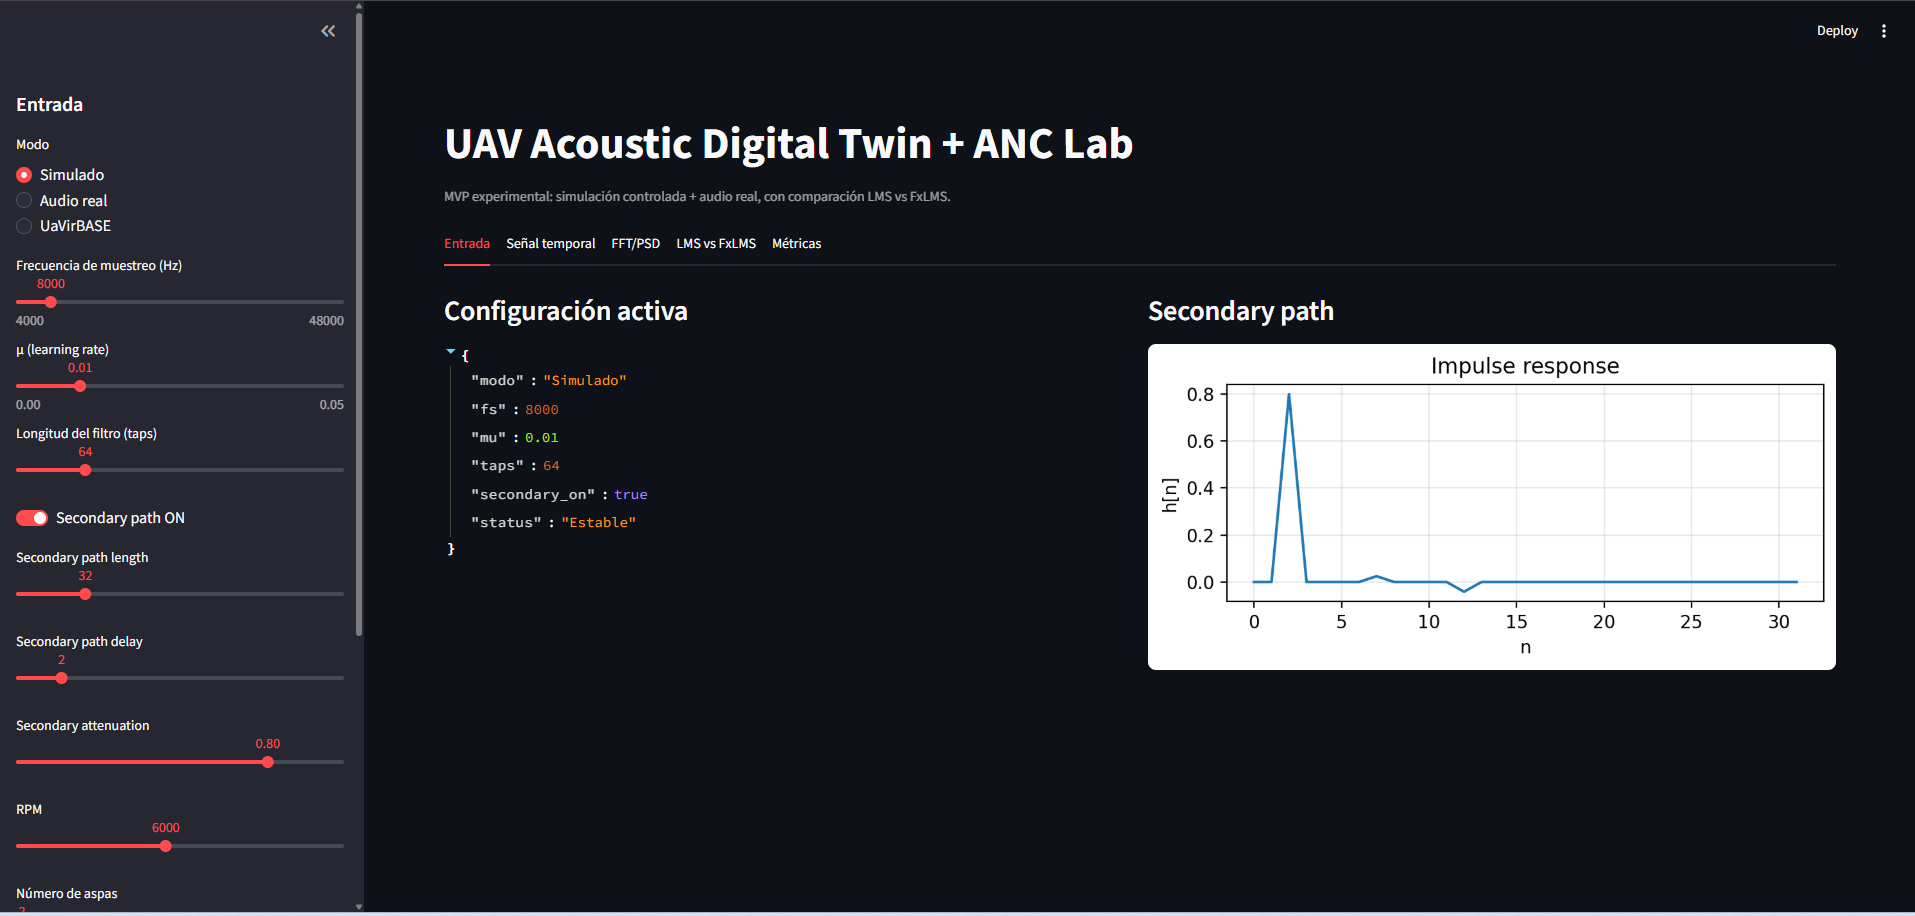
\includegraphics[width=\columnwidth]{01_config.png}
  \caption{Panel de configuración interactivo. Parámetros: RPM, número de
           palas, $\mu$, coeficientes del filtro, activación y geometría
           del camino secundario.}
  \label{fig:config}
\end{figure}

\subsection{Fase 1 — Validación de Línea de Base con LMS}

La Tabla~\ref{tab:lms} reporta la reducción de ruido en función de $\mu$.
La tasa de adaptación $\mu=0{,}01$ logra el mejor equilibrio
velocidad--estabilidad, obteniendo $\Delta_{\text{RR}} = \SI{24,53}{dB}$
con convergencia en aproximadamente \SI{0,5}{s}.
A $\mu=0{,}05$ el algoritmo diverge (NaN), confirmando el límite
teórico superior.

\begin{table}[t]
  \centering
  \caption{Rendimiento del LMS en función de la Tasa de Adaptación
           ($L=64$, $f_s=\SI{8}{kHz}$, $T=\SI{2}{s}$)}
  \label{tab:lms}
  \begin{tabular}{@{}lrrr@{}}
    \toprule
    $\mu$ & Reducción (dB) & Convergencia & Estabilidad \\
    \midrule
    0,001 & 16,60          & $\sim$\SI{5}{s} & Estable \\
    \textbf{0,01}  & \textbf{24,53} & $\sim$\SI{0,5}{s} & \textbf{Óptimo} \\
    0,05  & N/A (diverge) & —          & Inestable \\
    \bottomrule
  \end{tabular}
\end{table}

La Fig.~\ref{fig:time_domain} ilustra la respuesta temporal antes y
después de la cancelación para $\mu=0{,}01$.

\begin{figure}[t]
  \centering
  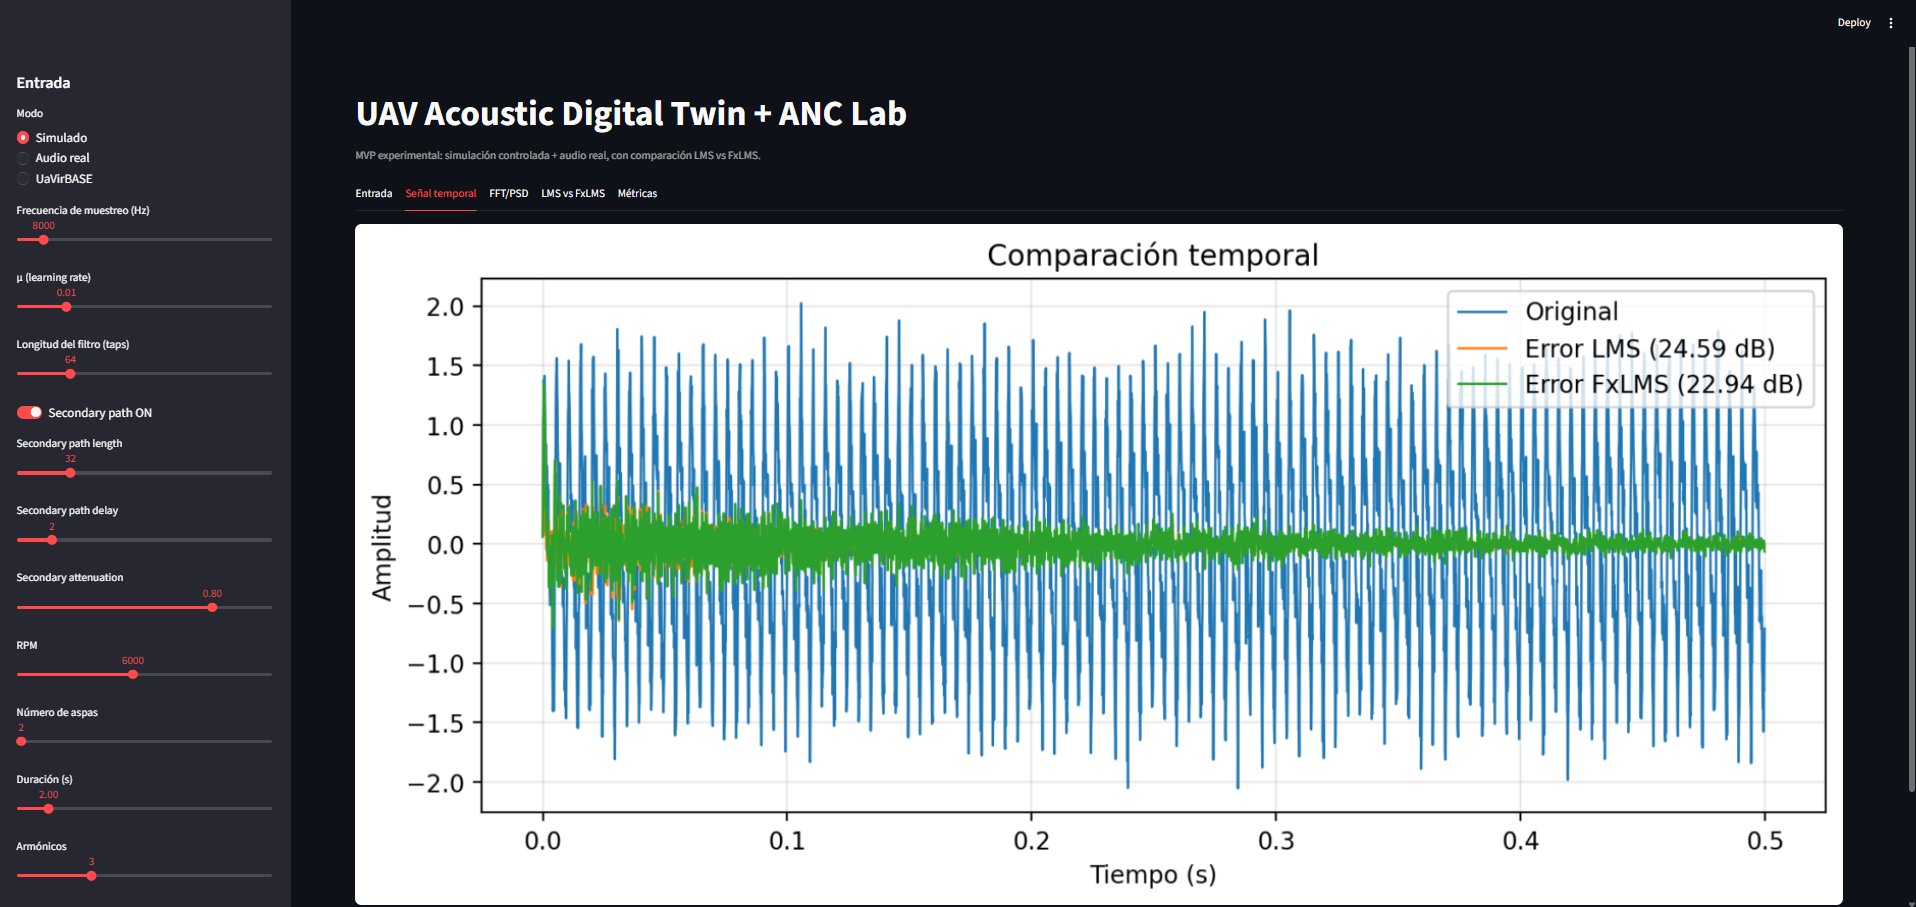
\includegraphics[width=\columnwidth]{02_time_domain.png}
  \caption{Comparación en el dominio temporal. Superior: señal de ruido
           UAV original; inferior: error residual tras la cancelación
           con LMS y FxLMS.}
  \label{fig:time_domain}
\end{figure}

Evolución del ECM:
\begin{itemize}
  \item \emph{ECM inicial:} $0{,}0307$
  \item \emph{ECM final (estado estacionario):} $0{,}0001$
  \item Reducción de cuatro órdenes de magnitud en $\sim\SI{0,5}{s}$.
\end{itemize}

\subsection{Fase 2 — FxLMS con Modelado del Camino Secundario}

La Fig.~\ref{fig:fft_psd} confirma la supresión espectral: tanto la FPP
(\SI{200}{Hz}) como el segundo armónico (\SI{400}{Hz}) se reducen a
magnitud cercana a cero en ambos algoritmos.

\begin{figure}[t]
  \centering
  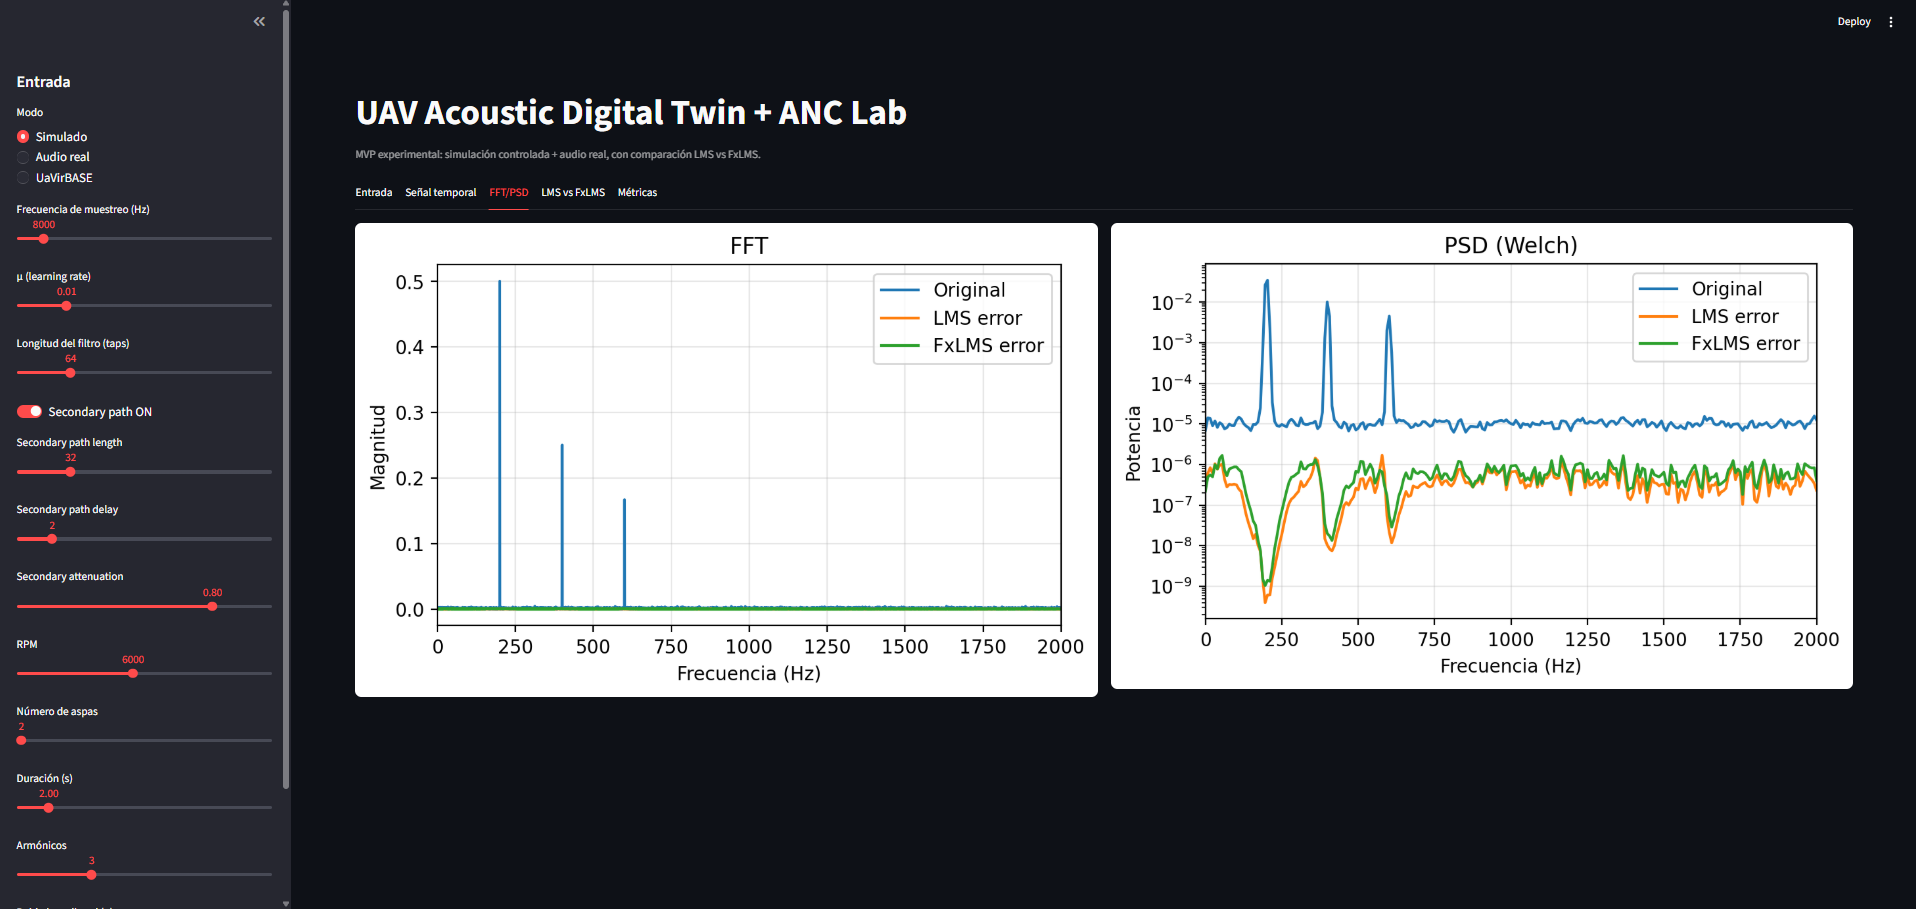
\includegraphics[width=\columnwidth]{03_fft_psd.png}
  \caption{Análisis en el dominio frecuencial. FFT (superior) y DEP
           (inferior) antes y después del CAR. La FPP y los armónicos
           quedan suprimidos en ambos algoritmos.}
  \label{fig:fft_psd}
\end{figure}

La Tabla~\ref{tab:compare} presenta la comparación pareada.
FxLMS alcanza \SI{22,83}{dB}, \SI{1,70}{dB} por debajo de LMS, como
consecuencia directa y cuantificable de tener en cuenta la dinámica
del camino secundario.

\begin{table}[t]
  \centering
  \caption{Comparativa LMS vs.\ FxLMS
           ($\mu=0{,}01$, $L=64$, camino secundario: $L_s=32$,
            $d=2$, $\alpha=0{,}8$)}
  \label{tab:compare}
  \begin{tabular}{@{}lrrrp{3.2cm}@{}}
    \toprule
    Algoritmo & $\Delta_{\text{RR}}$ (dB) & ECM$_0$ & ECM$_\infty$ & Observación \\
    \midrule
    LMS (ideal)            & 24,53 & 0,0307 & 0,0001 & Acoplamiento perfecto \\
    \textbf{FxLMS (real)}  & \textbf{22,83} & 0,0316 & 0,0002 & \textbf{Robusto} \\
    Diferencia             & $-1{,}70$ & — & — & Costo de robustez \\
    \bottomrule
  \end{tabular}
\end{table}

La Fig.~\ref{fig:convergence} muestra las curvas de ECM acumulado para
ambos algoritmos en paralelo, y la Fig.~\ref{fig:metrics} resume el
panel final de métricas de rendimiento.

\begin{figure}[t]
  \centering
  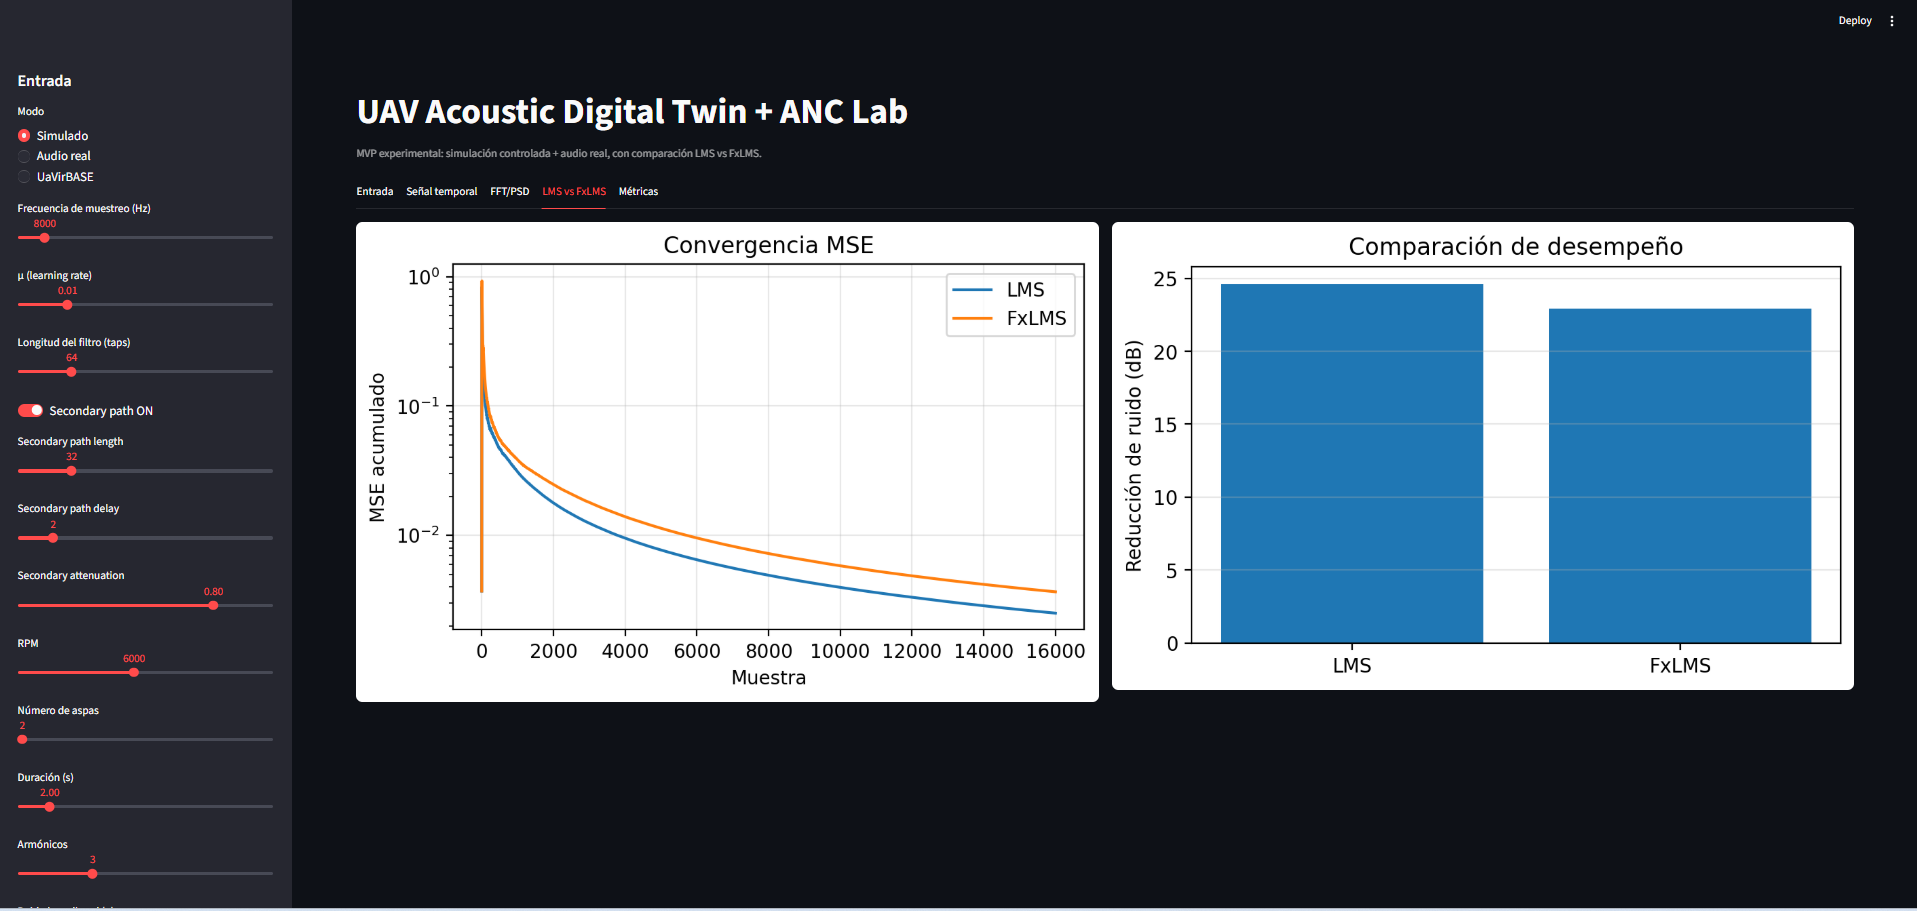
\includegraphics[width=\columnwidth]{04_convergence.png}
  \caption{Curvas de convergencia del ECM. LMS (azul) converge más rápido;
           FxLMS (naranja) converge a un suelo ligeramente mayor debido al
           filtrado del camino secundario.}
  \label{fig:convergence}
\end{figure}

\begin{figure}[t]
  \centering
  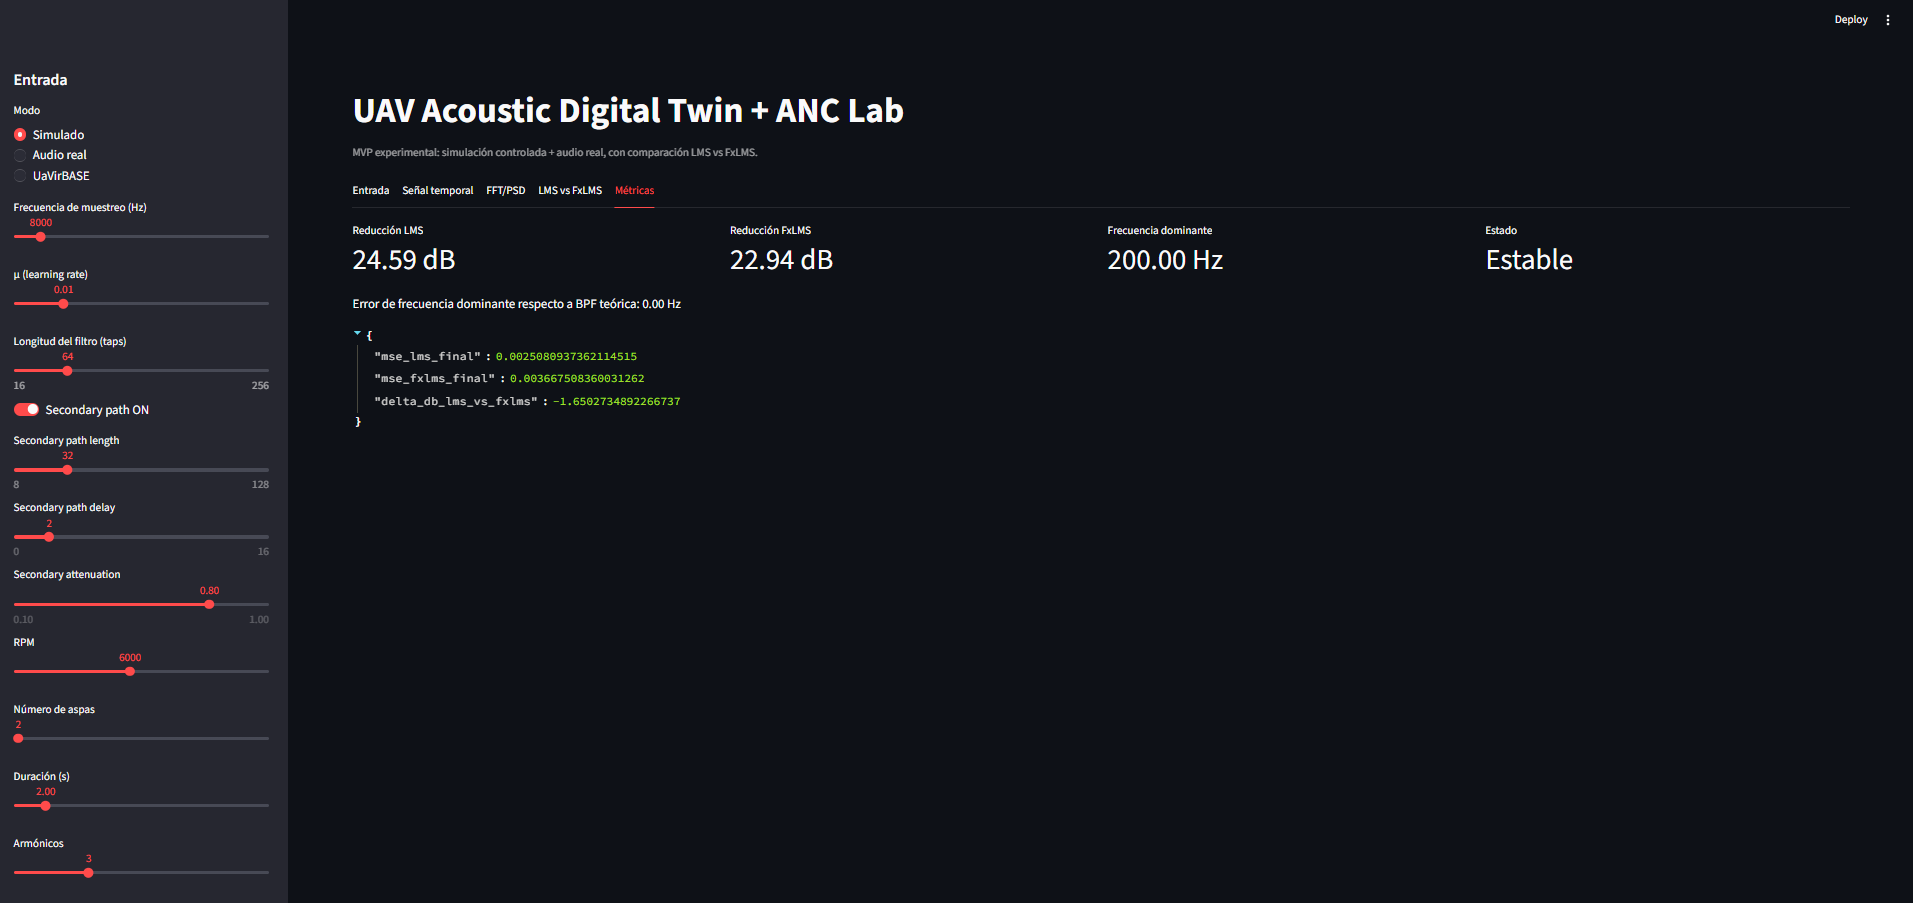
\includegraphics[width=\columnwidth]{05_metrics.png}
  \caption{Panel de métricas finales: reducción de ruido por algoritmo,
           frecuencia dominante estimada y estado de estabilidad.}
  \label{fig:metrics}
\end{figure}

% ─────────────────────────────────────────────────────────────
\section{Discusión}
\label{sec:discussion}

\subsection{El compromiso LMS--FxLMS}

La diferencia de \SI{1,70}{dB} entre LMS y FxLMS no es un fallo de
FxLMS, sino el \emph{costo esperado de la robustez}.
LMS asume implícitamente que la función de transferencia del camino de
cancelación es unitaria; cualquier desfase introducido por el camino
secundario alinea incorrectamente la estimación del gradiente, lo que
puede causar divergencia en canales reales.
FxLMS corrige esto pre-filtrando la referencia con el camino secundario
estimado, garantizando actualizaciones de gradiente con signo correcto
a costa de un paso de convergencia ligeramente menor.

\subsection{Análisis del Margen de Estabilidad}

La divergencia observada a $\mu=0{,}05$ es consistente con la condición
de estabilidad Nyquist--LMS:
\begin{equation}
  \mu < \frac{2}{\lambda_{\max} L}
\end{equation}
Para la señal BPF sintética con potencia normalizada y $L=64$,
$\lambda_{\max}\approx 1$, situando el límite teórico en
$\mu\approx 0{,}031$, lo que enmarca la divergencia observada.

\subsection{Validación en el Dominio Frecuencial}

La supresión de la FPP a \SI{200}{Hz} y del armónico a \SI{400}{Hz}
confirma que el filtro adaptativo modela la estructura tonal del ruido.
El ruido de banda ancha residual (suelo de ruido blanco) no es afectado,
lo cual es consistente con la teoría CAR feedforward: sólo se cancela
el componente correlacionado observable en el micrófono de referencia.

\subsection{Limitaciones y Alcance}

El marco actual opera sobre señales mono y estacionarias.
La operación real de un UAV introduce FPP variable en el tiempo
(variaciones de RPM durante maniobras), interferencia acústica
multi-rotor y entornos exteriores con alta reverberación, todo lo cual
queda fuera del alcance actual y constituye extensiones naturales del trabajo.

% ─────────────────────────────────────────────────────────────
\section{Conclusión}
\label{sec:conclusion}

Este trabajo presentó un marco de referencia reproducible, orientado a la
simulación, para evaluar algoritmos CAR feedforward sobre ruido de hélices
UAV.
El filtro LMS alcanzó \SI{24,53}{dB} de reducción de ruido a $\mu=0{,}01$
con un filtro de $L=64$ coeficientes, y FxLMS alcanzó \SI{22,83}{dB}
bajo un modelo realista del camino secundario—una diferencia cuantificada
de \SI{1,70}{dB} que representa el costo de la robustez.
El análisis espectral confirmó la supresión de la FPP dominante a
\SI{200}{Hz} y del armónico a \SI{400}{Hz} en ambos casos.

El framework se implementa como una librería Python completamente de código
abierto con una interfaz interactiva Streamlit que soporta señales
sintéticas, entrada WAV real y un cargador de conjunto de datos acústico
UAV (compatible con UaVirBASE).
El trabajo futuro incluye: (i) integración del conjunto de datos UaVirBASE
real para validación hardware-en-el-lazo, (ii) simulación espacial de CAR
con \texttt{pyroomacoustics}, (iii) extensiones NLMS/RLS en tiempo real,
y (iv) despliegue embebido en plataformas DSP/FPGA.

% ─────────────────────────────────────────────────────────────
\appendix
\section*{Apéndice: Parámetros de Simulación}
\label{app:params}

\begin{table}[h]
  \centering
  \caption{Parámetros por defecto de la simulación}
  \begin{tabular}{@{}lll@{}}
    \toprule
    Parámetro & Símbolo & Valor \\
    \midrule
    Frecuencia de muestreo     & $f_s$      & \SI{8000}{Hz} \\
    Duración de la señal        & $T$        & \SI{2}{s} \\
    Número de palas            & $B$        & 2 \\
    Velocidad del rotor        & $\Omega$   & \SI{6000}{RPM} \\
    Frecuencia de paso de pala & $f_{\text{FPP}}$ & \SI{200}{Hz} \\
    Número de armónicos        & $K$        & 3 \\
    Desv.\ est.\ ruido broadband & $\sigma$  & 0,2 \\
    Orden del filtro           & $L$        & 64 coef. \\
    Tasa de adaptación         & $\mu$      & 0,01 \\
    Longitud camino secundario & $L_s$      & 32 coef. \\
    Retardo camino secundario  & $d$        & 2 muestras \\
    Atenuación camino sec.     & $\alpha$   & 0,8 \\
    \bottomrule
  \end{tabular}
  \label{tab:params}
\end{table}

% ─────────────────────────────────────────────────────────────
\bibliographystyle{IEEEtran}
\begin{thebibliography}{10}

\bibitem{widrow1985}
B.~Widrow y S.~D.~Stearns,
\emph{Adaptive Signal Processing}.
Englewood Cliffs, NJ: Prentice-Hall, 1985.

\bibitem{kuo1996}
S.~M.~Kuo y D.~R.~Morgan,
\emph{Active Noise Control Systems: Algorithms and DSP Implementations}.
Nueva York: Wiley, 1996.

\bibitem{elliott2001}
S.~J.~Elliott,
\emph{Signal Processing for Active Control}.
Londres: Academic Press, 2001.

\bibitem{nelson1992}
P.~A.~Nelson y S.~J.~Elliott,
\emph{Active Control of Sound}.
Londres: Academic Press, 1992.

\bibitem{kuo1999}
S.~M.~Kuo y D.~R.~Morgan,
``Active noise control: a tutorial review,''
\emph{Proc.\ IEEE}, vol.~87, no.~6, pp.~943--973, jun.\ 1999.

\bibitem{shi2020}
D.~Shi, B.~Lam y C.~Gan,
``Practical implementation of multichannel filtered-x least mean square
algorithm based on the multiple-parallel-branch with folding architecture
for active noise control of impulsive noise,''
\emph{IEEE Trans.\ Ind.\ Electron.}, vol.~67, no.~7,
pp.~5686--5695, jul.\ 2020.

\bibitem{torija2022}
A.~Torija, R.~Torija e I.~Ruiz,
``UAV noise characterization and metrics,''
\emph{Appl.\ Acoust.}, vol.~195, 2022, Art.\ no.~108850.

\bibitem{strauss2023}
M.~Strauss \emph{et al.},
``Active acoustic noise cancellation for small unmanned aerial vehicles:
design and evaluation,''
\emph{Aerospace}, vol.~10, no.~3, 2023.

\bibitem{yoo2023}
C.~B.~Yoo \emph{et al.},
``Simulation-first methods for adaptive system validation,''
en \emph{Proc.\ IEEE Int.\ Symp.\ Signal Process.}, pp.~1--8, 2023.

\bibitem{kuo2006}
S.~M.~Kuo, S.~Mitra y W.-S.~Gan,
``Active noise control system for headphone applications,''
\emph{IEEE Trans.\ Control Syst.\ Technol.}, vol.~14, no.~2,
pp.~331--335, mar.\ 2006.

\end{thebibliography}

\end{document}
